\section{Realistic domain simulation}

In this section we test the idea of implementing equivalent linear method on heterogenous medium.  We study the Mw 6.7 1994 Northridge, California, earthquake with a simulation domain with a volume domain of $81.92 km*81.92 km*40.96 km$, which includes the entire San
Fernando Valley and some of the Los Angeles metropolitan area. \citet{isbiliroglu2015coupled} used the earthquake and simulation domain to study the coupled soil-structure interaction effects of building clusters during earthquakes. They simulated earthquake with $Vs_{min}=200 m/s$ and $f_{max}=5~Hz$. They used extended source model provided by \citet{graves2010broadband}. In this study we use the same simulation domain, however, we use updated source model (reference). Figure.~\ref{fig:northridge_simulation_domain_stations_temp} shows the study domain, source model, and station location:

 \begin{figure}[h]
    \centering
    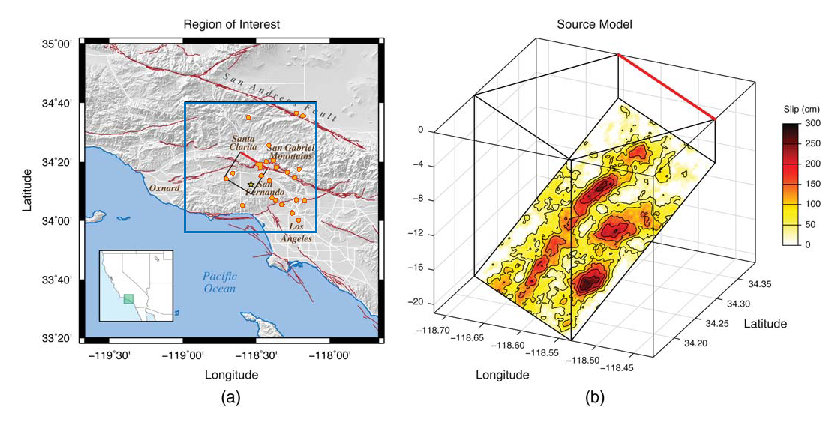
\includegraphics[width=\textwidth]{figures/pdf/northridge_simulation_domain_stations_temp.pdf}
    \caption{Simulation domain}
    \label{fig:northridge_simulation_domain_stations_temp}
\end{figure}


The observation data is according to the SCEC broadband platform validation exercise \citep{goulet2014scec}.

Stations record (signal)
PGV plane
Response spectra of the plan 


